<<<<<<< HEAD:Documentation/General/productVision/productVision.tex
\chapter{Introduction}

When people want to party, they want to listen to loud bass-heavy hype music.
When people feel down, they want to listen to slower emotional music.
When people feel sleepy, they want to listen to calm music.
The type of music people want to listen to is based on their mood, there's no doubt about that.

Our goal is to use this relationship between mood and music,
combine it with a music recommendation system and make a music service
that will influence and be influenced by the listeners over time.

Besides, we will add a social component to listening mood based music.
It does not matter which genre a song belongs to or which mood a listener is in; 
listening music together is more joyful, since you can share experiences.
We want to make a music service that connects people that are in the same mood and make them enjoy the songs together.
Users of our music service will be able to join a room based on a chosen mood.
This room will also have a chat to be able to interact with other people who are in the same mood.

Listeners will provide feedback on the change of music by clicking buttons to (dis)like songs.
This feedback will influence the song-selection system to further enhance the future user experience.

The combination of a mood-based song-selection algorithm and a chat to be able to interact with other users makes MoodCat a successful product.
These crucial components will satisfy the previously defined goal and will therefore be our main focus point of development.

\section{Timeframe}
This product will be developed over a span of 11 weeks, with no budget.
% That is, besides the daily pie budget.
Every week will consist of a sprint which will result in a working product to be shown at the demonstration on fridays.

\chapter{Why should we build MoodCat?}
=======
\documentclass[10pt,a4paper]{article}
\usepackage[utf8]{inputenc}
\usepackage{amsmath}
\usepackage{amsfonts}
\usepackage{amssymb}
\usepackage{cite}
\usepackage{hyperref}
\usepackage{graphicx}
\usepackage{siunitx}

\begin{document}

\title{Product Vision\\
	\begin{small}
	The why, who and what
	\end{small}
}
% Question: should this be our names or organization name?
\author{MoodCat.me}
\maketitle

\subsection*{Preface}

When people want to party they loud bass-heavy hype music.
When people feel down they want to listen to slower emotional music.
When people feel sleepy they want to listen to calm music.
What music people listen is based on their mood, there's no doubt about that.

There is, however, another side to this relationship between mood and music.
Not only do people want to listen music related to the mood they're in,
music can actively change the mood of the listener.
When people listen to loud bass-heavy hype music, people do get hyped,
people do get sad when listening to sad music,
sleepy music makes people sleepy.

Our goal is to use this bidirectional relationship between mood and music,
combine it with a music recommendation system and make a music service
that will influence and be influenced by the listener's mood over time.
This is our main focus point.

Besides this we're going to add a social component to listening mood based music.
It doesn't matter which genre, which mood, listening music is always more powerful if you can do it together.
We want to make a music service that connects people that are in the same mood, and make them enjoy their moods together.
Users of our music service will be able to join a room based on a chosen mood and chat and listen music along with other people with the same mood.

The general idea of rooms is that the room's mood changes over time, new songs will be put forward programatically. Happy rooms might slowly 
transition to relaxed rooms or maybe move towards louder music. Listeners will provide feedback on the change of music through like and dislike
buttons and together this will be a concretion of the mood/music relation.

Our service will is all about mood combined with social interaction through the Internet. Cats rule the internet like this MoodCat has been born.

\section{Why should we build MoodCat?}
>>>>>>> master:Documentation/General/productVision/productVision.tex
Various competitors provide a system that can offer users popular songs or songs that are similar to songs the user already listened to.
These recommendations mostly consist of songs that are popular or users with simmilar preferences listened to.
This leaves a huge amount of music produced by a lot of artists undiscovered.

Secondly, most music platforms do not offer user interaction in the form either chat or messaging systems.
By voting songs up or down, users influcence the system and mostly their personal recommendations from the system: the suggestion list is built indirectly using user information.
These suggestions are derived from song history and voting behaviour.

Some competitors offer users rooms to socialize while experiencing songs.
An example is Plug DJ \cite{PlugDJ} where users can create a room and listeners can suggest Youtube-songs\cite{Youtube} for the playlist.
Such a playlist has to be maintained in order to keep running and therefore does not suit the listeners that want to listen on their own.
Furthermore, it has to be moderated to prevent unwanted suggestions that might not be interesting for the listeners.

\bigskip 

Users want to discover music and have social interaction.
MoodCat allows users (and friends!) to unite in rooms, and listen to and discuss music together.
Hereby we apply a successful feature from the live video/gaming streaming industry (for example TwitchTV \cite{Twitch}) to the music industry.
Music rooms never fall silent, instead they are continuously filled with relevant music that fits the mood of the listeners in the room.

\chapter{What is the target audience of MoodCat?}
Our target audience consists of everyone who wants to listen to new songs based on their current mood.
More specifically, the users of MoodCat will mainly consist of people who want to discover songs they have not heard yet.
In the data-mining field this is also known as \textit{fetching from the long tail}\cite{longtail}.
By offering songs that match the users mood, the user will be satisfied with the music suggestions while also having the possibility of discovering new and unknown - yet interesting - music.
With this we can offer a unique user experience.

\chapter{What are the selling points of MoodCat?}
MoodCat has several selling points that would make it unique in the current music market.

\begin{enumerate}
\item The system is able to offer relevant songs using the specified current mood of the user.

\item MoodCat offers users both to experience solely or communicate with fellow music listeners.

\item The service can be used no matter how many other users are currently online.
This is achieved by making MoodCat self-maintaining.

\item With MoodCat unknown or lesser known artists have equal chances to let their songs be played.
This is a result of the system choosing songs based on features and is therefore unbiased regarding play counts.

\item MoodCat can determine mood trends of a user and can adjust the room-ordering and song-selection mechanisms accordingly.

\end{enumerate}

\chapter{Which components should MoodCat have?}
MoodCat will be developed as three separate componentents: the frontend, the backend and a special music matching algorithm.

\begin{enumerate}
\item The frontend will be the visible part for the listener.
The user will be able to select his mood and based on that MoodCat will provide several music listening rooms.
The user can select a room and immediately start listening to the currently played song.
In these rooms, after logging in, the user can interact with other listeners through the chat while listening to the music.

\item The backend keeps track of which rooms are active and what song is currently played in the room.
Furthermore, the backend is responsible for transmitting the chat messages between the users in the room.

\item The music matching algorithm is used to compare and match moods of songs and chatrooms.
It has two roles: list the room suggestions for a user and provide the next song to be played for a room.
\end{enumerate}

\newpage

\subsection{Frontend}

The MoodCat frontend will be web-based.
This allows us to support all modern devices which enables a large target audience.
We will develop the frontend using modern techniques as HTML5\cite{HTML}, CSS3\cite{CSS} and AngularJS\cite{AngularJS}.
Users can login using their Soundcloud account.
This allows us to integrate with the Soundcloud platform and prevents having to register for our services first.

\subsection{Backend}

The MoodCat backend will be a RESTful\cite{rest} API written in Java using JAX-RS. It will be backed by a relational (PostgreSQL) database. The backend connects the frontend to the music matching algorithm.

\subsection{Music matching algorithm}

The Music matching algorithm determines and compares moods for songs, rooms and users.
Moodcat will be developed around a learning algorithm.
This means that Moodcat will improve over time.
Default values will be determined by examining the audio features provided by our data set.
Then, through a system of user votes, the system will learn and improve over time.

We discovered that moods and emotions can be mapped to a valence/arousal plane\cite{Yang:2006:MEC:1180639.1180665} (see figure \ref{fig:avgraph}).

\begin{figure}[h]
\center
<<<<<<< HEAD:Documentation/General/productVision/productVision.tex
\includegraphics[scale=0.75]{avgraph.jpg}
\caption{The valence/arousal graph \cite{Book}}
=======
\includegraphics[scale=0.75]{../avgraph.jpg}
\caption{The valance/arousal graph \cite{Book}}
>>>>>>> master:Documentation/General/productVision/productVision.tex
\endcenter
\label{fig:avgraph}

\end{figure}

Arousal and valence are psychological terms\cite{Thayer}.
Arousal means how calm or excited you are.
Valence is the amount of attraction you have towards a certain event.

In order to use arousal and valence, we have to express them in terms of music features.
For valence we can use harmony, mode and tonality\cite{DianaDeutsch}.
For arousal we can use pitch, timbre \cite{Liu03automaticmood}, speed and loudness \cite{PresentationMER}\cite{PaperME}.

\newpage

The data provided by the Multimedia Computing group from EEMCS does not explicitly provide the above features.
However, we can extract some of them from the low-level features the data does provide.

The low-level features we can use for valence:
\begin{enumerate}
\item For harmony we can use the consonance and dissonance of a song.
\item To determine the mode of a song, we can use the key, key scale and key strength from the data.
The key strength also tells a bit about the tonality of the song.
When the key strength approaches 1, we can speak of tonality. When the key strength approaches 0, we can speak of atonality.
\end{enumerate}
The low-level features we can use for arousal:
\begin{enumerate}
\item Beats-per-minute (BPM) gives us the tempo of a song.
\item Loudness can be directly retrieved from the loudness feature.
\item Pitch can be derived from the tuning frequency, which is standardized at \SI{440}{\hertz} but may vary depending on music genre, era and geography.
\end{enumerate}

The timbre of a song is a separate research field and would be too difficult to integrate into our system.

<<<<<<< HEAD:Documentation/General/productVision/productVision.tex
Using the above features, we will tweak a song-classifier algorithm that can determine the mood of a song given a set of features.
Tweaking the algorithm will be done by personal preference of the team members and later on with the input of the system users.
=======
%
% BIBLIOGRAPHY
%
\bibliography{productVision}{}
\bibliographystyle{plain}

\end{document}
>>>>>>> master:Documentation/General/productVision/productVision.tex
